\clearpage
\chapter{音阶与调式}

\classquote{宫为君，商为臣，角为民，徵为事，羽为物。五者不乱，则无怗懘之音矣。}{《礼记·乐记·乐本》}{五声各有位置与角色，次序一乱，声音就不顺。调式也是这样：先选一个主音，再让其余音围绕它排成有中心的音阶。古人用政治作比喻，你只需记住“音阶内部要有稳定关系”。}

\label{chap:scales-and-modes}

\subsection*{学完这一章能做什么}
\begin{itemize}
  \item 用“全—全—半—全—全—全—半”写出任意大调音阶，并说清七个音级各叫什么。
  \item 分清自然小调、和声小调、旋律小调，知道升七级会带来什么听觉变化。
  \item 看懂调号与五度圈，能把 C 大调与 A 小调这类“关系大小调”对上。
  \item 写出五声音阶与七种常见调式，并在夜半的钢琴卷帘上按半音行距把它们摆出来。
\end{itemize}

\subsection{音阶：把半音排成有主次的阶梯}

音阶（scale）是一个八度内按音高排序的一组音。它不只是“一串音名”，而是有主音的等级结构：\textbf{主音}（tonic）是这套音的中心，其余音按与主音的距离获得不同的功能。音阶里的每一个位置叫\textbf{音级}（scale degree），用 1–7 编号；第 8 个音回到主音，只是高一个八度。

七个音级的常用名字：

\begin{center}
\small
\begin{tabular}{cll}
\toprule
音级 & 中文名 & English \\
\midrule
1 & 主音 & tonic \\
2 & 上主音 & supertonic \\
3 & 中音 & mediant \\
4 & 下属音 & subdominant \\
5 & 属音 & dominant \\
6 & 下中音 & submediant \\
7 & 导音（小调自然七级为下主音） & leading tone / subtonic \\
\bottomrule
\end{tabular}
\end{center}

音阶的“形状”可以用相邻音之间的半音数描述。两个半音叫全音（whole tone），一个半音还是半音（semitone）。大调与小调的区别，主要就在这串“全/半”的排列顺序，以及主音落在哪里。

\subsection{大调音阶}

从 C4 开始，按“全、全、半、全、全、全、半”走，得到 C 大调：

\[
\mathrm{C4 \xrightarrow{+2} D4 \xrightarrow{+2} E4 \xrightarrow{+1} F4
\xrightarrow{+2} G4 \xrightarrow{+2} A4 \xrightarrow{+2} B4 \xrightarrow{+1} C5}
\]

用音级写就是 \(1\ 2\ 3\ 4\ 5\ 6\ 7\ 8\)，相邻音级之间的半音数依次是 \(2,2,1,2,2,2,1\)。这个公式对任何主音都成立：把 C 换成 D，就从 D 开始按同样的步子走，得到 D 大调；换成 F，就得到 F 大调。

大调的两个关键位置是主音到中音（1–3，四个半音，大三度）和主音到属音（1–5，七个半音，纯五度）。这两段距离稳定，听感上把“家”和“支柱”定住。第七级到主音只差一个半音，所以叫导音（leading tone）：它天然指向主音，旋律停在导音上会有“没唱完”的感觉。

\begin{figure}[htbp]
\centering
\begin{tikzpicture}[x=1.45cm,y=0.40cm,font=\scriptsize]
  \foreach \i/\n/\h in {0/C4/0,1/D4/2,2/E4/4,3/F4/5,4/G4/7,5/A4/9,6/B4/11,7/C5/12} {
    \draw[gray] (\i,-0.35) -- (\i,\h);
    \node[above=3pt] at (\i,\h) {\n};
  }
  \draw[very thick] (0,0) -- (1,2) -- (2,4) -- (3,5) -- (4,7) -- (5,9) -- (6,11) -- (7,12);
  \foreach \i/\lab/\yy in {0/全/1.15,1/全/3.15,2/半/4.75,3/全/6.15,4/全/8.15,5/全/10.15,6/半/11.75} {
    \node[font=\scriptsize,fill=white,inner sep=1.5pt,above=1pt] at (\i+0.5,\yy) {\lab};
  }
\end{tikzpicture}

\small 图 4-1：C 大调的“阶梯”。折线高度是该音相对 C4 的半音数；折线旁标注相邻两音的全/半关系，最后一步 B4–C5 只差一个半音。
\end{figure}

\subsection{小调：自然、和声、旋律}

小调也由一个主音和七个音级组成，但三级与六级比同名大调低一个半音，听感更暗、更内敛。最常见的是 A 自然小调（A natural minor）：从 A3 起按 \(2,2,1,2,2,1,2\) 走，得到

\[
\mathrm{A3\ B3\ C4\ D4\ E4\ F4\ G4\ A4}.
\]

它的音名集合与 C 大调完全相同，只是主音从 C 换成了 A。这就是“关系大小调”：同一组音、同一个调号，主音不同，功能与听感就不同。A 自然小调的第七级 G 到主音 A 差两个半音，不构成导音，所以 G 叫下主音（subtonic），而不是导音。

和声小调（harmonic minor）把自然小调的第七级升高一个半音：A 和声小调是 A B C D E F G\sharpsym{} A。这个升七级制造了两个效果：G\sharpsym{} 到 A 变成半音，重新获得导音；F 到 G\sharpsym{} 变成三个半音，出现小调特有的增二度（augmented second）。增二度听起来有张力，常被用来写小调的“招牌”旋律。

旋律小调（melodic minor）进一步处理六级和七级：上行时把 F、G 都升高（A B C D E F\sharpsym{} G\sharpsym{} A），让旋律更顺畅；下行时通常回到自然小调的 F、G。不同教材对下行的处理有差异，但“上行升六、七级，下行还原”是最常见的口径。

\begin{center}
\small
\begin{tabular}{p{0.18\linewidth}p{0.40\linewidth}p{0.30\linewidth}}
\toprule
类型 & A 主音音阶 & 关键差别 \\
\midrule
自然小调 & A B C D E F G & 七级为下主音，无增二度 \\
和声小调 & A B C D E F G\sharpsym & 升七级，F–G\sharpsym{} 为增二度 \\
旋律小调 & 上行 A B C D E F\sharpsym{} G\sharpsym；下行回 F、G & 上行升六、七级，下行常还原 \\
\bottomrule
\end{tabular}

表 4-1：三种小调。实际写作中和声小调最常用，旋律小调多用于声乐或旋律经过句。
\end{center}

\subsection{调号与五度圈}

调号（key signature）是记谱时写在谱号后面的一组升号或降号，用来省略音阶中反复出现的升降记号。它不改变音高体系，只是把“这套音阶要升/降哪些音级”写成约定。

升号的书写顺序固定为 F、C、G、D、A、E、B；降号顺序固定为 B、E、A、D、G、C、F。记住顺序比死背每个调更重要：看到三个升号，就知道是 F\sharpsym、C\sharpsym、G\sharpsym；看到两个降号，就是 B\flatsym、E\flatsym。

把常用大调按“主音上行纯五度”排开，就得到五度圈（circle of fifths）的一条展开线：

\begin{figure}[htbp]
\centering
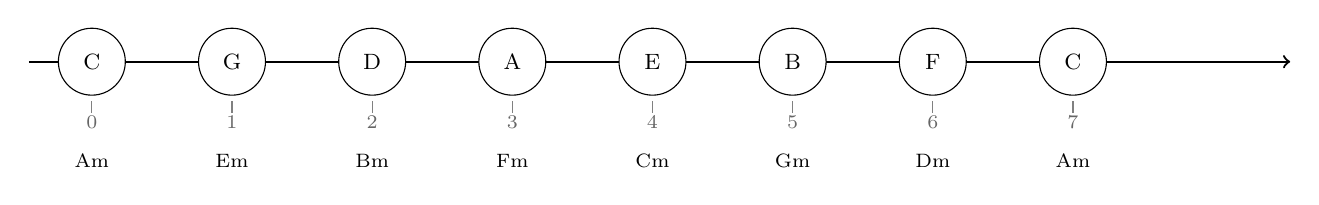
\begin{tikzpicture}[x=1.78cm,y=1cm,font=\footnotesize]
  \draw[->,thick] (-0.45,0) -- (8.55,0);
  \foreach \i in {0,...,7} {\draw[gray] (\i,-0.5) -- (\i,-0.65);}
  \node[circle,draw,fill=white,minimum size=0.85cm,inner sep=0pt] (c0) at (0,0) {C};
  \node[circle,draw,fill=white,minimum size=0.85cm,inner sep=0pt] (c1) at (1,0) {G};
  \node[circle,draw,fill=white,minimum size=0.85cm,inner sep=0pt] (c2) at (2,0) {D};
  \node[circle,draw,fill=white,minimum size=0.85cm,inner sep=0pt] (c3) at (3,0) {A};
  \node[circle,draw,fill=white,minimum size=0.85cm,inner sep=0pt] (c4) at (4,0) {E};
  \node[circle,draw,fill=white,minimum size=0.85cm,inner sep=0pt] (c5) at (5,0) {B};
  \node[circle,draw,fill=white,minimum size=0.85cm,inner sep=0pt] (c6) at (6,0) {F\sharpsym};
  \node[circle,draw,fill=white,minimum size=0.85cm,inner sep=0pt] (c7) at (7,0) {C\sharpsym};
  \foreach \i/\sig in {0/0,1/1\sharpsym,2/2\sharpsym,3/3\sharpsym,4/4\sharpsym,5/5\sharpsym,6/6\sharpsym,7/7\sharpsym} {
    \node[below=16pt,font=\scriptsize,text=black!60] at (\i,0) {\sig};
  }
  \foreach \i/\mn in {0/{Am},1/{Em},2/{Bm},3/{F\sharpsym m},4/{C\sharpsym m},5/{G\sharpsym m},6/{D\sharpsym m},7/{A\sharpsym m}} {
    \node[below=30pt,font=\scriptsize] at (\i,0) {\mn};
  }
\end{tikzpicture}

\small 图 4-2：五度圈展开线。向右每走一格，主音上行纯五度，升号多一个；圆圈下方是调号，再下方是对应的关系小调。反向走则降号增加，F 大调为 1 个降号，B\flatsym{} 大调为 2 个，依此类推。
\end{figure}

调号相同的大调与小调互为关系大小调。C 大调与 A 小调都是 0 个升降号；G 大调与 E 小调都是 1 个升号；F 大调与 D 小调都是 1 个降号。关系小调的主音在大调主音下方小三度（或上方大六度），例如 C 下方小三度是 A。

不要把它和“同主音大小调”混淆：C 大调与 C 小调主音相同、调号不同，叫同主音大小调（parallel major/minor）；C 大调与 A 小调主音不同、调号相同，叫关系大小调（relative major/minor）。

\subsection{五声音阶}

五声音阶（pentatonic scale）只取五个音级，天然避开了一些半音冲突。最常见的大调五声音阶取大调的 1、2、3、5、6 级，也就是省掉 4 级和 7 级：

\[
\mathrm{C4\ D4\ E4\ G4\ A4}.
\]

C 宫系统在传统音乐里写作宫、商、角、徵、羽，对应 C、D、E、G、A；以 A 为羽就是 A 羽调式，音集仍是这五个音。小调五声音阶取 1、\(\flat\)3、4、5、\(\flat\)7 级：

\[
\mathrm{A3\ C4\ D4\ E4\ G4}.
\]

五声音阶的稳定性来自“没有半音相邻”：C 大调五声里相邻音至少隔两个半音，旋律不容易撞到尖锐的半音冲突。它适合快速写出民歌风、流行副歌或 riff；需要更丰富的和声时，再把省掉的 4、7 级加回去。

\subsection{常用调式}

调式（mode）可以理解为“同一条大调音阶，换一个音当主音”。以 C 大调的七个音为材料，分别以 C、D、E、F、G、A、B 为主音，就得到七种调式。也可以用“从主音出发的半音公式”直接重建。七种调式的常见中文译名依次是伊奥尼亚、多利亚、弗里吉亚、利底亚、混合利底亚、爱奥利亚、洛克里亚。

\clearpage
\begin{center}
\footnotesize
\renewcommand{\arraystretch}{1.12}
\setlength{\tabcolsep}{3pt}
\begin{longtable}{p{0.17\linewidth}p{0.37\linewidth}p{0.25\linewidth}p{0.15\linewidth}}
\toprule
调式 & 以 C 为主音的音阶 & 半音公式 & 特征 \\
\midrule
\endhead
Ionian & C D E F G A B & 2,2,1,2,2,2,1 & 就是大调 \\
Dorian & C D E\flatsym{} F G A B\flatsym & 2,1,2,2,2,1,2 & 小调但六级为自然六度 \\
Phrygian & C D\flatsym{} E\flatsym{} F G A\flatsym{} B\flatsym & 1,2,2,2,1,2,2 & 降二级，开头沉重 \\
Lydian & C D E F\sharpsym{} G A B & 2,2,2,1,2,2,1 & 升四级，明亮悬浮 \\
Mixolydian & C D E F G A B\flatsym & 2,2,1,2,2,1,2 & 大调但七级为降七级 \\
Aeolian & C D E\flatsym{} F G A\flatsym{} B\flatsym & 2,2,1,2,2,1,2 & 自然小调 \\
Locrian & C D\flatsym{} E\flatsym{} F G\flatsym{} A\flatsym{} B\flatsym & 1,2,2,1,2,2,2 & 降二、降五，最不稳定 \\
\bottomrule
\end{longtable}

表 4-2：七种调式。表里给的是“以 C 为主音”的写法，方便比较；实际使用时主音可以换，公式不变。
\end{center}

调式的“味道”通常由一个或两个特征音决定：Dorian 的 \(\sharp\)6（相对自然小调升高六级）、Phrygian 的 \(\flat\)2、Lydian 的 \(\sharp\)4、Mixolydian 的 \(\flat\)7、Locrian 的 \(\flat\)2 与 \(\flat\)5。写旋律时，先把这个特征音放在能听见的位置，调式才立得住；只换主音而不碰特征音，听感会模糊。

\subsection{在夜半里怎么做}

\begin{enumerate}
  \item 打开钢琴卷帘（\texttt{P}/\texttt{F7}）。卷帘相邻一行是一个半音，所以可以直接用行距写音阶：C 大调从 C4 行起，依次放在 +0、+2、+4、+5、+7、+9、+11、+12 行，得到 C4 D4 E4 F4 G4 A4 B4 C5。
  \item 写 A 自然小调时，从 A3 行起放 +0、+2、+3、+5、+7、+8、+10、+12 行；要听和声小调，把第七级 G 改成 G\sharpsym（向上移一行），再播放对比。
  \item 顶部走带栏的 \texttt{KEY / SCALE} 读数只在一个三预设循环里切换（C Minor 自然小调、D Dorian 多利亚、F Major 大调），点击会改工程的调号元数据；它不会把卷帘行自动染成音阶音级，也不支持任意调式选择。练本章调式时，以卷帘上手动摆出的音为准，别把这个读数当成完整的调式工具。
  \item 听关系大小调：用同一组白键音（C D E F G A B），第一个版本从 C 开始、重拍落在 C；第二个版本从 A 开始、重拍落在 A。音高材料没变，主音一变，听感就从“大调”转向“小调”。
  \item 写五声音阶：C 大调五声只留 C4、D4、E4、G4、A4，删掉 F4 与 B4；A 小调五声留 A3、C4、D4、E4、G4。需要更密的和声时再加回被省掉的音。
  \item 所有音高判断以 A4 = 440 Hz 为参照；听调式时先校准监听音量与播放速度，不要凭记忆硬判。
\end{enumerate}

\screenshot{piano-roll-scale-ladder}{卷帘中的音阶阶梯}

\textbf{范围说明：}夜半当前没有“按调式自动铺音阶/标音级”的专门面板；顶部 \texttt{KEY / SCALE} 只有三个预置读数，且不驱动卷帘着色。本章的操作步骤都按“手动摆音＋行距核对”写，不指向不存在的音阶生成按钮。

\subsection{练习}


\begin{exercise}
\begin{enumerate}
  \item 写出 C 大调的七个音级与相邻半音数；B4 到 C5 是几个半音？\\
  \emph{答案：}C D E F G A B；半音数 \(2,2,1,2,2,2,1\)；B4–C5 是 1 个半音。

  \item 写出 A 自然小调的音名与关系大调；把第七级升高后得到什么小调？被升高的是哪个音？\\
  \emph{答案：}A B C D E F G；关系大调是 C 大调；升高 G 得到 A 和声小调。

  \item 三个升号的调号对应哪两个关系大小调？主音分别是谁？\\
  \emph{答案：}A 大调（A）与 F\sharpsym{} 小调（F\sharpsym）；升号是 F\sharpsym、C\sharpsym、G\sharpsym。

  \item C 大调五声音阶包含哪些音？省掉了哪两个音级？A 小调五声音阶又包含哪些音？\\
  \emph{答案：}C D E G A；省掉 4 级 F 与 7 级 B；A 小调五声是 A C D E G。

  \item 在夜半里从 D4 起写出 D Dorian 的七个音，并说明它与 C 大调的关系。\\
  \emph{提示：}D Dorian 用 C 大调的音、以 D 为主音：D E F G A B C；在卷帘上从 D4 行起按 +0、+2、+3、+5、+7、+9、+10 行摆放，最后一个 C 在 C5（D4 的 +10 行）。\\
  \emph{答案：}D E F G A B C；音集与 C 大调相同，主音换成 D，六级 B 为自然六度，是 Dorian 的标志。
\end{enumerate}
\end{exercise}

\subsection{帮助主题映射}

\begin{center}
\footnotesize
\setlength{\tabcolsep}{3pt}
\begin{longtable}{p{0.34\linewidth}p{0.45\linewidth}p{0.15\linewidth}}
\toprule
本章小节 & 应用内帮助锚点 & 备注 \\
\midrule
\endhead
音阶与音级 & \texttt{music-theory-scale-degrees} & 概念 \\
大调音阶 & \texttt{music-theory-major-scale} & 图 4-1 \\
小调三种形态 & \texttt{music-theory-minor-scales} & 表 4-1 \\
调号与五度圈 & \texttt{music-theory-key-signature-circle} & 图 4-2 \\
关系大小调 & \texttt{music-theory-relative-keys} & 概念 \\
五声音阶 & \texttt{music-theory-pentatonic} & 公式 \\
常用调式 & \texttt{music-theory-modes} & 表 4-2 \\
在夜半里怎么做 & \texttt{music-theory-piano-roll-scales} & 操作 \\
练习 & \texttt{music-theory-ch4-practice} & 答案在章末 \\
\bottomrule
\end{longtable}
\end{center}

\subsection*{延伸阅读}
\begin{itemize}
  \item \textbf{Open Music Theory, “Scales and scale degrees.”} \url{https://openmusictheory.github.io/scales.html} —— 从音级与主音讲大小调、调式与调号，补本章的体系感。
  \item \textbf{YouTube, “Modes and Scales” playlist.} \url{https://www.youtube.com/playlist?list=PLlx2eo2tD6KoGvA_q0DFrYeLuwklZEy0O} —— 用真实歌曲逐条对照七种调式的听感，避免只背音阶。
\end{itemize}

